%%%%%%%%%%%%%%%%%%%%%%%%%%%%%%%%%%%%%%%%%%%%%%%%%
%       Macroscopic analysis of load curve      %
%   Antoine                                     %
%%%%%%%%%%%%%%%%%%%%%%%%%%%%%%%%%%%%%%%%%%%%%%%%%
\subsection{Macroscopic analysis of a load curve}
We need a fast algorithm that can be called at any moment to detect a device based on the load curve. In case the results of this approach are doubtful, then microscopic algorithms are used.

The macroscopic algorithms are based on the differenciate function, which helps detect a jump in the load curve. Indeed the difference between two point of a jump is directly the consumption of the device, as shown in \ref{fig1} where the grouped square are a heater use.

\begin{figure}[H]
\centering
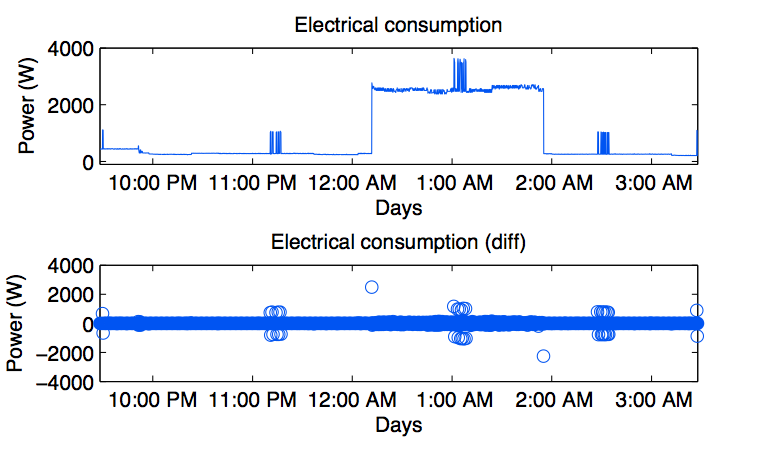
\includegraphics[scale=0.8]{figures/fig_antoine_5.png}
\caption{Example of a real load curve}
\label{fig1}
\end{figure}

We define several steps of consumption: 100, 500 and 750W which mean for small consulption device (such as lights), medium consumption (oven) and heavy consumption (heater). The load curve reaching one of these values means the device is turning on, and reaching the same negative value means the device is turning off. With this basic approach we can define some devices, but we cannot differenciate an unknow device consuming 500W from an oven for example.

Therefore, we developped a second algorithm that analyzes the signature load curve of each device. Every devices have a specific and unic load curve when they turn on and if we can create a data base with these signatures, then we can determine which device has just turn on. Spotting when the devices turn off is simple as it corresponds to negative values of the differenciate function.

An example will help make the description clearer. A heater power consumption load curbe is basically a a square repetition. This shape is due to the periodicity of the device. By detecting such a wave form in the load curve, then we can detect heater consumption and estimate the consumption of this device. We obtain the following result shown on the figure \ref{fig2}.


\begin{figure}[H]
\centering
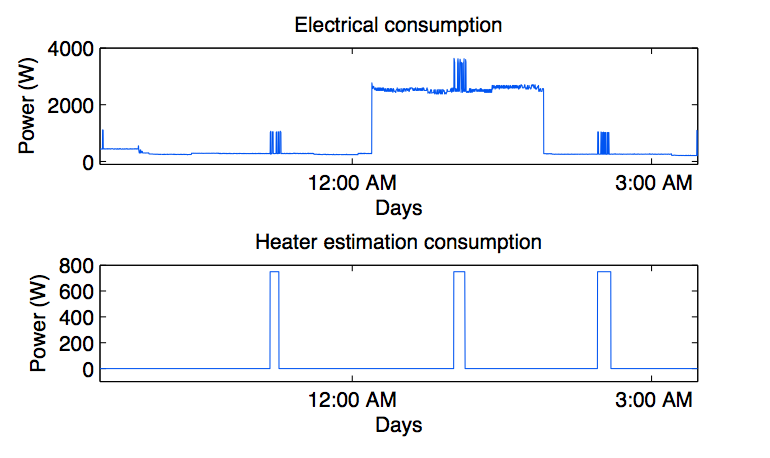
\includegraphics[scale=0.8]{figures/fig_antoine_6.png}
\caption{Estimation of a heater consumption}
\label{fig2}
\end{figure}


We proceed in the same way for non periodical devices such as a dishwasher or a washing machine. But for instant, only the dishwasher has been implemented.


